%\documentclass{ijsra}
\def\IJSRAidentifier{\currfilebase} %<---- don’t change this!
%-------Title | Email | Keywords | Abstract-------------
\def\shorttitle{A damage- and risk-assessment of Petra}
\def\maintitle{The Crumbling Wonder: A damage- and risk-assessment of sandstone monuments and natural features in the Petra Archaeological Park (Jordan)}
\def\cmail{V.Verezen@gmail.com}
\def\keywords{Archaeology, Heritage Preservation, Safety-Risks,  Nabataean, Weathering, Monuments}
%\def\keywordname{}%<--- redefine the name “Keywords“ in needed language
\def\abstract{Petra, famous for its monumental archaeology, is in danger: it is ‘crumbling’. This fragile sandstone wonder has fallen victim to degradation. This research sheds light on the deterioration of valuable archaeology in the Petra Archaeological Park. It is aimed to clarify the factors contributing to this decay and the need for active and continuous protection. Additionally, it highlights specific monuments and natural features within the archaeological park which require attention regarding their deterioration and safety-risks. Protecting Petra equally means the safeguarding of perishable data. Through reviewing Petra’s geo-archaeological data, applying safety regulations, and conducting extensive risk- and damage-assessments, its archaeology and safety can be maintained.}
%--------Author’s names------------
\def\authorone{Valletta Aretti Maria Verezen}
%-------Biographical information-------------
\def\bioone{\href{https://leidenuni.academia.edu/VallettaVerezen}{Valletta Verezen} % (Leidschendam-Voorburg; 23-03-1990) 
is an Archaeologist from the Netherlands who graduated from Leiden University in February 2016. She specialises in the Archaeology of the Near and Middle East, particularly Nabatean culture, heritage studies, and archaeobotany. She has conducted fieldwork at Jebel-Qurma (Azraq, Jordan) and at Udruh, a Nabataean / Roman legionary fortress and outpost in the hinterland of Petra, located along ancient caravan-trade routes and the Via Traiana Nova. She currently lives in the Bedouin village of Petra (Umm Sayhoun), studying the rich history of this ancient monument. With her work, Valletta aims to raise awareness about the fragile state of preservation of Petra in dire need of protection in order to safeguard its future.
Her specializations are in Near Eastern archaeology, botany, and osteoarchaeology. 
%	http://www.linkedin.com/in/vallettaverezen
}
%------University/Institution--------------
\def\affilone{Graduate Archaeologist, Leiden University}

\begin{filecontents}{\IJSRAidentifier.bib}
%these top 2 references need to be fixed from here

@Article{alsaad2001,
  author       ={Al-Saad, Z. and M. Abdel-Halim},
  title        ={Laboratory evaluation of various types of mortars for the conservation of Qasr al-Bint monument, Petra-Jordan},
  volume       ={23},
  pages        ={926--933},
  date         ={2001},
  journaltitle ={Engineering Structures},
}

@Article{alshawabkehy2010,
  author       ={Alshawabkeh, Y. and F. Bala’awi},
  title        ={3D Digital Documentation, Assessment and Damage Quantification of the Al-Deir Monument in the Ancient City of Petra, Jordan},
  volume       ={12},
  number       ={2},
  pages        ={124--145},
  date         ={2010},
  journaltitle ={Conservation and Management of Archaeological Sites},
}

@Article{alweshahr1999,
  author       ={Al-Weshah, R.A. and F. El-Khouri},
  title        ={Flood Analysis and Mitigation for Petra Area in Jordan},
  volume       ={125},
  number       ={3},
  pages        ={170--177},
  date         ={1999},
  journaltitle ={Journal of Water Resources Planning and Management},
}

@TechReport{assante1993,
  author      ={Assante di Panzillo, C. and B. Bousquet and C. Jouffray and B. Lane and P. Laureano and A. Ohannessian-Charpin and J. Rewerski and F. Zayadine},
  title       ={Draft Management Plan for Petra Archaeological and Natural Park},
  institution ={UNESCO},
  date        ={1993},
  location    ={Paris},
}

@InProceedings{balaawi2011,
  author       = {Balaáwi, F. and Alawneh, F. and Alshawabkeh, F. and Waheeb, M.},
  title        = {Conservation Work at Petra: What has been done and what is needed},
  booktitle    = {Proceedings from the International Conference: Conservation of Architecture, Urban Areas, Nature \& landscape Towards a Sustainable Survival of Cultural Landscape},
  volume       = {2},
  pages        = {267--284},
  organization = {The Centre for Study of Architecture in the Arab Region},
  publisher    = {CSAAR Press},
  date         = {2011},
  location     = {Amman, Jordan},
}

@Article{bille2012,
  author       ={Bille, M.},
  title        ={Assembling Heritage: Investigating the UNESCO Proclamation of Bedouin Intangible Heritage in Jordan},
  volume       ={18},
  pages        ={107--123},
  date         ={2012},
  journaltitle ={International Journal of Heritage Studies},
}

@InProceedings{comer2011,
  author       = {Comer, D. and W. Willems},
  title        = {Tourism and Archaeological Heritage. Driver to Development or Destruction?},
  booktitle    = {Proceedings of the 17\textsuperscript{th} ICOMOS General Assembly. Aces du Symposium de la XVIIème assemblee generale de l’ICOMOS organisée par ICOMOS France},
  editor       = {Gottfried, C. and S. Hidalgo},
  volume       = {17},
  pages        = {499--511},
  organization = {ICOMOS},
  publisher    = {ICOMOS},
  date         = {2011},
  location     = {Paris},
}

@Book{comer2012,
  title     ={Tourism and Archaeological Management at Petra: Driver to Development or Destruction?},
  publisher ={Springer},
  author    ={Comer, D.},
  date      ={2012},
  location  ={New York},
}

@InCollection{delmonaco2013,
	author       ={Delmonaco, G. and Margottini, C. and Spizzichino, D.},
	title        ={Rock-Fall Hazard Assessment in the Siq of Petra, Jordan},
	booktitle    ={Risk-Assessment, Management and Mitigation},
	publisher    ={Springer Berlin Heidelberg},
	editor       ={Margottini, C. and Canuti, P. and Sassa, K.},
	volume       ={6},
	series       ={Landslide Science and Practice},
	pages        ={441--446},
	date         ={2013},
	organization ={The Second World Landslide Forum},
}

@InCollection{doehne2002,
  author       ={Doehne, E.},
  title        ={Salt Weathering: A Selective Review},
  booktitle    ={Natural Stone, Weathering Phenomena, Conservation Strategies and Case Studies},
  publisher    ={Geological Society of London},
  editor       ={Siegesmund, S and  S. Vollbrecht and T. Weiss},
  volume       ={205},
  series       ={Geological Society, London, Special Publication},
  pages        ={51--64},
  date         ={2002},
  organization ={Geological Society of London},
}

@Article{fhb03,
  author       ={Fitzner, B. and Heinrichs, K. and La Bouchardiere, D.},
  title        ={Weathering Damage on Pharaonic Sandstone Monuments in Luxor-Egypt},
  volume       ={38},
  pages        ={1089--1103},
  date         ={2003},
  journaltitle ={Building and Environment},
}

@Article{franchi2009,
  author       ={Franchi, R. and Savelli, D. and Colosi, F. and Drapp, P. and Gabrielli, R. and Moretti, E. and Peloso, D.},
  title        ={Petra and Beida (Jordan): two adjacent archaeological sites up to an exploitation of geomorphology-related topics for a cultural and touristic development},
  volume       ={87},
  pages        ={77--90},
  date         ={2009},
  journaltitle ={Memorie descrittive della carta geologica dítalia},
}

@Booklet{harding1938,
  title        ={Hashemite Kingdom of Jordan, Petra; A Brief History and Some Photographs},
  author       ={Harding, G.},
  howpublished ={Through the Department of Antiquities (Amman, Jordan) and Clowes (London, UK)},
  date         ={1938},
  location     ={Amman, Jordan},
}

@Article{heinrichs2008,
  author       ={Heinrichs, K.},
  title        ={Diagnosis of Weathering Damage on Rock-Cut Monuments in Petra, Jordan},
  volume       ={56},
  pages        ={643--675},
  date         ={2008},
  journaltitle ={Environmental Geology},
}

@InProceedings{heinrichs2013a,
  author       = {Heinrichs, K. and Azzam, R.},
  title        = {Investigation of salt weathering on stone monuments – the ‘petraSalt’ research project},
  booktitle    = {Proceedings of the 19\textsuperscript{th} Conference on Engineering Geology and of the Forum for Young Engineering Geologists},
  editor       = {K. Thuro},
  volume       = {19},
  pages        = {347--352},
  organization = {Technische Universität München},
  publisher    = {Technische Universität München},
  date         = {2013-03},
  location     = {Munich},
}

@InProceedings{heinrichs2013b,
  author       = {Heinrichs, K. and R. Azzam},
  title        = {Damage associated with geological discontinuities on rock-cut monuments in Petra / Jordan},
  booktitle    = {Proceedings of the 19\textsuperscript{th} Conference on Engineering Geology and of the Forum for young Engineering Geologists},
  editor       = {K. Thuro},
  volume       = {19},
  pages        = {583--588},
  organization = {Technische Universität München},
  publisher    = {Technische Universität München},
  note         = {2\textsuperscript{nd} article of K. Heinrichs and R. Azzam in the 19\textsuperscript{th} proceeding},
  date         = {2013},
  location     = {Munich},
}

@Www{icomos2004-2005,
  date ={2004/2005},
  url  ={http://www.icomos.org/risk/2004/jordan2004.pdf},
}

@InProceedings{icomos2005,
 author = {ICOMOS},
 title = {Jordan: Petra},
 booktitle = {Heritage at Risk 2004/2005},
 pages = {151--156},
 date = {2005},
 url = {http://www.icomos.org/risk/2004/jordan2004.pdf}
}

@Article{lingis2002,
  author       = {Lingis, A.},
  title        = {Petra},
  volume       = {1},
  number       = {1},
  pages        = {47--55},
  date         = {2002},
  journaltitle = {Journal of Visual Culture},
}

@Book{maqsood1994,
  title     = {Petra, A Travellerś Guide},
  publisher = {Bell and Bain Ltd.},
  author    = {Maqsood, R.},
  edition   = {first},
  date      = {1994},
  location  = {Glasgow (UK)},
}

@Article{matyscak2014,
  author       = {Matyšcák, O. and Ottosen, L. and I. Rörig-Dalgaard},
  title        = {Desalination of salt damaged Obernkirchen sandstone by an applied DC field},
  volume       = {71},
  pages        = {561--569},
  date         = {2014},
  journaltitle = {Construction and Building Materials},
}

@Article{mckenzie1991,
	author       = {McKenzie, J.},
	title        = {The Beduin at Petra: The Historical Sources},
	volume       = {23},
	number       = {1},
	pages        = {139--145},
	date         = {1991},
	journaltitle = {Levant},
}

@Article{mustafa2011,
	author       = {Mustafa, M.H. and Abu Tayeh, S.N.},
	title        = {The Impacts of Tourism Development on the Archaeological Site of Petra and Local Communities in Surrounding Villages},
	volume       = {7},
	number       = {8},
	pages        = {88--96},
	date         = {2011},
	journaltitle = {Asian Social Sciences},
}

@Article{mustafa2013,
  author       = {Mustafa, M.H. and Bala’awi, F.},
  title        = {Evaluating Visitor Management at the Archaeological Site of Petra},
  volume       = {13},
  number       = {1},
  pages        = {77--87},
  date         = {2013},
  journaltitle = {Mediterranean Archaeology and Archaeometry},
}

@Book{nichols2009,
  title     = {Sedimentology and Stratigraphy},
  publisher = {Wiley-Blackwell},
  author    = {Nichols, G.},
  edition   = {2},
  date      = {2009},
  location  = {Oxford (UK)},
}

@Article{ortloff2005,
  author       = {Ortloff, C.R.},
  title        = {The Water Supply and Distribution System of the Nabataean City of Petra (Jordan), 300 BC–AD 300},
  volume       = {15},
  number       = {1},
  pages        = {93--109},
  date         = {2005},
  journaltitle = {Cambridge Archaeological Journal},
}

@Book{paolini2012,
  title     = {Risk Management at Heritage Sites; A Case Study of the Petra World Heritage Site},
  publisher = {UNESCO},
  author    = {Paolini, A. and Vafadari, A. and Cesaro, G. and Quintero, M. and Van Balen, K. and Vileikis, O. and L. Fakhoury},
  date      = {2012},
}

@Article{papamichos2010,
  author       = {Papamichos, E.},
  title        = {Erosion and Multiphase Flow in Porous Media},
  volume       = {14},
  number       = {8-9},
  pages        = {1129--2254},
  date         = {2010},
  journaltitle = {European Journal of Environmental and Civil Engineering},
}

@Article{paradise1995,
  author       = {Paradise, T.},
  title        = {Sandstone Weathering Thresholds in Petra, Jordan},
  volume       = {16},
  pages        = {205--222},
  date         = {1995},
  journaltitle = {Physical Geography},
}

@Article{paradise2010,
  author       = {Paradise, T.},
  title        = {Sandstone Chamber Humidity and Tourism in Petra, Jordan},
  volume       = {16},
  number       = {2},
  pages        = {63--79},
  date         = {2010},
  journaltitle = {Journal of Architectural Conservation},
}

@Article{paradise2013,
  author       = {Paradise, T.},
  title        = {Assessment of tafoni distribution and environmental factors on a sandstone djinn block above Petra, Jordan},
  volume       = {42},
  pages        = {176--185},
  date         = {2013},
  journaltitle = {Applied Geography},
}

@Article{peterman1994,
  author       = {Peterman, G.},
  title        = {Archaeology in Jordan},
  volume       = {98},
  number       = {3},
  pages        = {521--559},
  date         = {1994},
  journaltitle = {American Journal of Archaeology},
}

@Article{rababeh2014,
  author       = {Rababeh, S. and H. Al-Qablan and S. Abu-Khafajah and M. El-Mashaleh},
  title        = {Structural utilization of wooden beams as anti-seismic and stabilising techniques in stone masonry in Qasr El-Bint, Petra, Jordan},
  volume       = {54},
  pages        = {60--69},
  date         = {2014},
  journaltitle = {Construction and Building Materials},
}

@Article{rörigdalgaard2015,
  author       = {Rörig-Dalgaard, I.},
  title        = {Further developments of a poultice for electrochemical desalination of porous building materials: minimization of side effects},
  volume       = {48},
  pages        = {1901--1917},
  date         = {2015},
  journaltitle = {Materials and Structures},
}

@InProceedings{sachet2010,
  author       = {Sachet, L.},
  title        = {Feasting with the Dead: Funerary Marzeah in Petra},
  booktitle    = {Death and Burial in Arabia and Beyond},
  editor       = {L. Weeks},
  volume       = {10},
  series       = {2107},
  pages        = {249--262},
  organization = {Multidisciplinary Perspective, Society for Arabian Studies Monograph},
  publisher    = {Archaeopress (BAR International Series)},
  date         = {2010},
  location     = {Oxford (UK)},
}

@Article{turkington2005,
  author       = {Turkington, A. and T. Paradise},
  title        = {Sandstone Weathering; a Century of Research and Innovation.},
  volume       = {68},
  pages        = {229--253},
  date         = {2005},
  journaltitle = {Geomorphology},
}

@TechReport{usicomos1996,
  author      = {US-ICOMOS},
  title       = {Management Analysis and Recommendations for the Petra World Heritage Site, Jordan},
  institution = {US-ICOMOS Jordan},
  type        = {Report},
  date        = {1996},
}

@Article{volkwein2011,
  author       = {Volkwein, A. and Schellenberg, K. and Labiouse, V. and Agliardi, F. and Berger, F. and Bourrier, F. and Dorren, L. and Gerber, W. and M. Jaboyedoff},
  title        = {Rockfall Characterisation and Structural Protection - A Review},
  volume       = {11},
  pages        = {2617--2651},
  date         = {2011},
  journaltitle = {Natural Hazards and Earth System Sciences},
}

@Www{wmpf1996-2016,
  date ={1996/2016},
  url  ={https://www.wmf.org/project/petra-archaeological-site},
}

@URL {worldmonumentsfund2017,
 author = {World Monuments Fund},
 title = {Petra Archaeological Site},
 date ={2017},
 url = {https://www.wmf.org/project/petra-archaeological-site},
}

@Article{young2003,
  author       = {Young, E. and Urquhart, D. and R. Laing},
  title        = {Maintenance and repair issues for stone cleaned sandstone and granite building façades},
  volume       = {38},
  pages        = {1125--1131},
  date         = {2003},
  journaltitle = {Building and Environment},
}

\end{filecontents}
\IJSRAopening%<---- don’t change this!
%-------
\lettrine{L}{ocated} \IJSRAsection{Introduction} in the south of Jordan is a marvellous ancient sandstone city carved by the Nabataeans known as Petra \pcref{fig:29-Verezen-figure-appendix01}.
This site lies adjacent to the Sharah Mountains and is located \num{265} kilometres South of Amman, Jordan’s capital city.
This archaeological wonderland was rediscovered in August 1812 by the Swiss explorer Johan Ludwig Burckhardt \parencite[1--5]{harding1938}. Beside European expeditions, much of its current fame has been contributed by the Hollywood block-buster movie \emph{Indiana Jones: The Last Crusade}.
In 1985, UNESCO listed Petra on the \emph{World Heritage List} which forced the local inhabitants\footnote{The local inhabitants of Petra are Bedouins known as the Al-Bdoul. Before being relocated to the government-built village of Umm Sayhoun, they were reusing ancient Nabataean caves as their homes. Some refused to be moved and remained on their tribal lands in Petra \parencites[108--110]{bille2012}[139--140]{mckenzie1991}[89]{mustafa2011}.} 
to relocate to the government-built village of Umm Sayhoun.
In 2007, Petra was nominated on the list of \emph{New Seven Wonders of the World}.
This acquired title gave a boost to the tourism-sector of Jordan.
Previously, the Petra Archaeological Park (PAP) received around \num{200000} visitors per year whereas after the acquired status it annually welcomed approximately \num{1000000} visitors \parencite[176]{paradise2013}.

Petra is a magnificent site, but unfortunately, great deterioration is affecting its future.
Therefore, its protection should be of increasing concern.
However, so far only three of the approximately 2000 monuments in Petra have been subjected to sandstone conservation\footnote{The extent to which conservation work can be conducted in Petra is highly dependent on the financial support from global funding agencies such as USAID 
\parencite[273--275]{balaawi2011}.} 
to prevent further decay 
\parencite[267-284]{balaawi2011}.
Having personally visited Petra, I was overwhelmed by its archaeology and sandstone rock formations.
However, upon spending one month in Petra, from July to August 2014, I started to observe the significant degradation, the negative impacts of mass tourism, natural weathering, and the unprotected status of the fragile and weathered monuments.
These basic observations were the principle beginnings for researching the current state of issues in Petra.
The purpose of this research is to clarify the vulnerability of the Petra Archaeological Park’s archaeology, to assess current safety-risks and suggest recommendations for the protection and preservation of the park’s archaeology.
In order to gain further understanding of the issues, I aim to answer the following research question: what factors cause the degradation of Petra’s archaeology and destabilization of natural features and could also pose safety-risks?
Additionally, what are the options to prevent further damage and to maintain safety in the archaeological park?  

The \IJSRAsection{Methodology} observed monumental destruction in Petra, during the first visit from July to August 2014, allowed for the realization of the disastrous effects of continuous weathering on the archaeological monuments.
Resulting from this, three monuments were selected as case studies based on their deteriorated condition \pcref{fig:29-Verezen-figure01,tab:Verezen-table1}, assessed by visual inspection, in the Petra Archaeological Park (PAP).
These monuments were chosen in order to reflect the impact of physical weathering present throughout Petra and the dire need for protection and conservation.
The visual inspections took place during 36 separate field-surveys spanning a 9-month period, from; September 2014 until June 2015, after already having visited Petra from the end of July until the end of August 2014.
The field-surveys took place in the Petra Archaeological Park and had an average duration of three days.
This 9-month time-span witnessed the shift from the winter to summer season and various weather extremities, such as heavy rainfall, snowfall, flash-floods and daily and seasonal temperature cycles.
Additionally, three possible hazardous natural features were selected in order to provide examples of the possible safety-risks in the Petra Archaeological Park \pcref{fig:29-Verezen-figure02,tab:Verezen-table2}.

\begin{table}[!htb]
	\centering
	\caption{Overview of the selected monuments. Their location (left column), name (middle), and state of degradation (right).}
	\label{tab:Verezen-table1}
	\begin{tabular}{|l|l|l|}
		\hline
		\textbf{Location}  & \textbf{Name}   & \textbf{State} \\ \hline
		Mu’Eissra Area     & Tomb 609        & Collapsed      \\ \hline
		Ad-Deir Mountain   & Monastery's Urn & Heavily Eroded \\ \hline
		El-Khubta Mountain & Corinthian Tomb & Heavily Eroded \\ \hline
	\end{tabular}
\end{table}

\begin{table}[!htb]
	\centering
	\caption{The selected natural and potential hazardous features inside the Petra Archaeological Park. Its location (left column), type (middle), and duration of its presence (right).}
	\label{tab:Verezen-table2}
	\begin{tabular}{|l|l|l|}
		\hline
		\textbf{Location}                                                                 & \textbf{Type}                                                                   & \textbf{Presence}                                                   \\ \hline
		The Treasury (Al-Khazneh)                                                         & \begin{tabular}[c]{@{}l@{}}Stuck boulder;\\ possible threat\end{tabular}        & Year-round                                                          \\ \hline
		Al-Habis Mountain                                                                 & \begin{tabular}[c]{@{}l@{}}Freestanding boulder;\\ possible threat\end{tabular} & Year-round                                                          \\ \hline
		\begin{tabular}[c]{@{}l@{}}Petra Archaeological Park\\ (entire area)\end{tabular} & Flash floods                                                                    & \begin{tabular}[c]{@{}l@{}}Seasonally;\\ mainly winter\end{tabular} \\ \hline
	\end{tabular}
\end{table}

While collecting visual data, there was an intention of selecting mainly the severely affected monuments that are lacking protection and conservation in regards to preservation.
During field-surveys, famous monuments were inspected such as; the Treasury (Al-Khazneh), the Monastery (Ad-Deir), the Qasr-al Bint (the Daughters Palace), and the Royal Tombs.
Additionally, more remotely located monuments were explored such as: the Triclinium, the Roman Soldier Tomb, the Turkmanniye Tomb, and various numbered tombs such as the collapsed Tomb 609 \pcref{fig:29-Verezen-figure-appendix02,fig:29-Verezen-figure01}.
Likewise, the selection of natural features in Petra was based on visual observation. This selection was based on the feature’s proximity to crowded areas, the park’s facilities, and archaeological structures.
These criteria were chosen in order to evaluate the safety-risk in case of its collapse.
The state, risks, and cause of degradation of the selected monuments and natural features were assessed through the conducted observations, inspections, and literature studies.
Various scholarly studies, regarding monumental degradation, likewise offered helpful insights in the factors affecting the deterioration of sandstone. 

The \IJSRAsection{Results: Degradation of Monuments} selected monuments offered a chance to determine the factors that are the most responsible for its sandstone decay.
These monuments also reflect the deteriorating situation of many other monuments in Petra.
The section below summarizes the factors causing degradation to the ancient monuments and affecting the natural features that could create potential safety-risks in the park.

Various \IJSRAsubsection{Weathering Factors} factors can cause physical weathering, a process responsible for the decay of bedrock and the removal and transportation of unconsolidated debris, known as regolith.
It is the breakdown of rock without triggering chemical reactions \parencite[90--92]{nichols2009}.
The factors causing physical weathering in Petra are: flash-floods, rain- and snow-fall, wind\footnote{Wind causes destruction in the form of wind-blown sand. This is known as wind-ablation and mainly abrades the base of monuments that come in touch with the airborne particles \parencite[267--284]{balaawi2011}.}, salt crystallization,
rising humidity-levels, seismic activities, anthropogenic activities, and daily temperature fluctuations, which cause expansion and
contraction of minerals, leading to rock-failure \parencites[126]{alshawabkehy2010}[667--669]{heinrichs2008}[90--97]{nichols2009}[12--14]{paolini2012}[66]{usicomos1996}.
During the field-surveys, a variety of these factors were observed and personally experienced, such as flash-floods, snow-fall, and heavy rain-fall.
The force of surface run-off water, deriving from rainfall, became clear upon observing the rapid formation of flash-floods and small waterfalls in the archaeological park. 

Surface run-off water removes and transports regolith, which abrades the sandstone surfaces \parencites[650--668]{heinrichs2008}[1130--1131]{papamichos2010}[207--208]{paradise1995}.
Furthermore, remaining water enters the porous sandstone and evaporates.
This evaporation causes the deposition of salt-crystals, which expand and widen existing fissures,
that can trigger rock-falls and monumental collapse.
This process is known as salt-wedging and is a great contributor to the degradation of Petra’s archaeology and
natural features \parencites[90]{nichols2009}[66]{usicomos1996}.
Salt-wedging, along with other weathering factors, undoubtedly contributed to the collapse of Tomb 609, which was inspected for this research. 

Vegetation is another factor contributing to the sandstone decay in Petra since rock-penetrating plant roots are known to
create and widen existing cracks  \parencites[125--126]{alshawabkehy2010}[230--242]{turkington2005}[66]{usicomos1996}.
There are likewise anthropogenic factors, or human activities, inflicting damage to Petra.
The increased tourism-flow has affected the local environment and enhanced the physical weathering of Petra’s geological features and
archaeology resulting from irresponsible tourist behaviour, such as illicit climbing activities \parencite[90]{mustafa2011}.

A consequence of the increased number of visitors is the rising humidity levels in Petra,
which significantly accelerates the decay of sandstone \parencite[75--76]{paradise2010}.
Throughout the field-surveys, unauthorized climbing activities were mainly observed at the Monastery where visitors and
locals would climb up the monument to sit at its Urn.
This activity, accompanied with visitors carving their names in the soft sandstone, afflicted considerable damage to the Monastery’s Urn.
The numerous tourist facilities have also affected Petra’s environment in terms of noise-pollution caused by
the facilities’ power-generators \parencite[88]{assante1993}.
Due to its vulnerable nature, Petra has several times been listed on the \emph{World Monument Watch List} for
endangered sites \parencites[58--62]{comer2012}[643]{heinrichs2008}[16]{paolini2012}{icomos2005}{worldmonumentsfund2017}.
 
Various \IJSRAsubsection{Tomb 609} collapsed monuments in Petra are the greatest examples and silent witnesses of the continuous forces of weathering and degradation.
The most recent example is Tomb 609 with the collapse of its façade \pcref{fig:29-Verezen-figure01} after heavy rainfall in March 2010,
known as the Mu’Eissra collapse \parencite[583]{heinrichs2013b}.
Tomb 609 followed a lengthy process of weathering through natural agents such as: water erosion, seasonal and daily temperature fluctuations,
salt-wedging and wind ablation, which caused physical stress and rock failure.
The rainfall was likely the last of a series of natural events causing its façade to collapse.

\begin{figure}[!htb]
	\includegraphics[width=\linewidth]{29-Verezen-figure01}
	\caption{The monuments assessed in this research.
		{\normalfont\scriptsize \\ \copyright\ by \shortauthor
	}}
	\label{fig:29-Verezen-figure01}
\end{figure}

This \IJSRAsubsection{The Monastery’s Urn} monument has the largest façade\footnote{The Monastery’s façade measures roughly 50 meters in width and 45 meters in height. The urn-like top is about 9.5 meters high \parencites[117--121]{maqsood1994}[129--130]{alshawabkehy2010}.}  in Petra and is known as the Monastery \parencite[117--121]{maqsood1994}.
The focus, regarding degradation, for this case-study was on the sculpted urn, which tops the monument.
Not observable from the front-view, is the severe deterioration of its South-East side \pcref{fig:29-Verezen-figure01}.
This side of the Urn has been eroded through natural weathering and anthropogenic activity.
During the field-surveys in Petra, locals and tourists were observed performing unauthorized climbing activities on this monument.
These illicit activities and irresponsible behaviours, occurring throughout the Petra Archaeological Park,
has created enhanced degradation \parencite[86]{paolini2012}.
The natural agents most affecting the Monastery itself are wind ablation, surface run-off water, salt-crystallization, and
vegetation \parencites[126--130]{alshawabkehy2010}[1--2]{doehne2002}.
These are the same factors damaging its Urn’s surface and structure.
Without intervention, the Urn will further deteriorate and this could lead to destabilisation and eventual collapse.
The latter will pose a threat to visitors of the Monastery. 

Another \IJSRAsubsection{The Corinthian Tomb} affected monument is part of the Royal Tombs, which are carved out of the Al-Khubta mountain.
The chosen monument is known as the Corinthian Tomb, the façade is extremely weathered and
resembles a water-damaged painting \parencite[257]{sachet2010}.
Various processes are responsible for the degradation of the Royal Tombs, such as: salt-wedging, surface run-off water,
vegetation, wind ablation, and tectonic movements \parencites[267--284]{balaawi2011}[1--3]{doehne2002}[90]{nichols2009}; icomos2005).
In the case of the Corinthian Tomb, surface run-off water and consequential salt-crystallization are the main contributors to
its façade’s decay and destabilization.
The latter could result in collapse; this is a threat to the integrity and safety of the souvenir shops, people, and
archaeology in its proximity.
Vegetation is another factor contributing to the deterioration of archaeological monuments \parencite[267--284]{balaawi2011}.
Likewise, vegetation is observed on the façade of the Corinthian Tomb and indicates that plant removal is necessary.
If degradation and the absence of protection continues, its façade might be unrecognizably weathered or collapsed in the future.

The \IJSRAsection{Results: Natural Features} chosen natural features of Petra shed light on the presence of possible hazards in the archaeological park that might threaten the integrity of the archaeology and the safety of visitors.

The \IJSRAsubsection{Treasury’s Boulder} first selection was a significant sandstone boulder stuck between a wedge-shaped fissure located to the upper-right side of the Treasury \pcref{fig:29-Verezen-figure02}.
The boulder is trapped in a rock-fissure; however, it could yet pose a safety-risk upon movement resulting from
significant surface run-off water or earthquakes.
Steel safety nets could be installed to catch falling debris upon collapse, because ignoring this risk could otherwise threaten the park’s safety and the Treasury’s façade \parencite[2617--2639]{volkwein2011}.

\begin{figure}[!htb]
	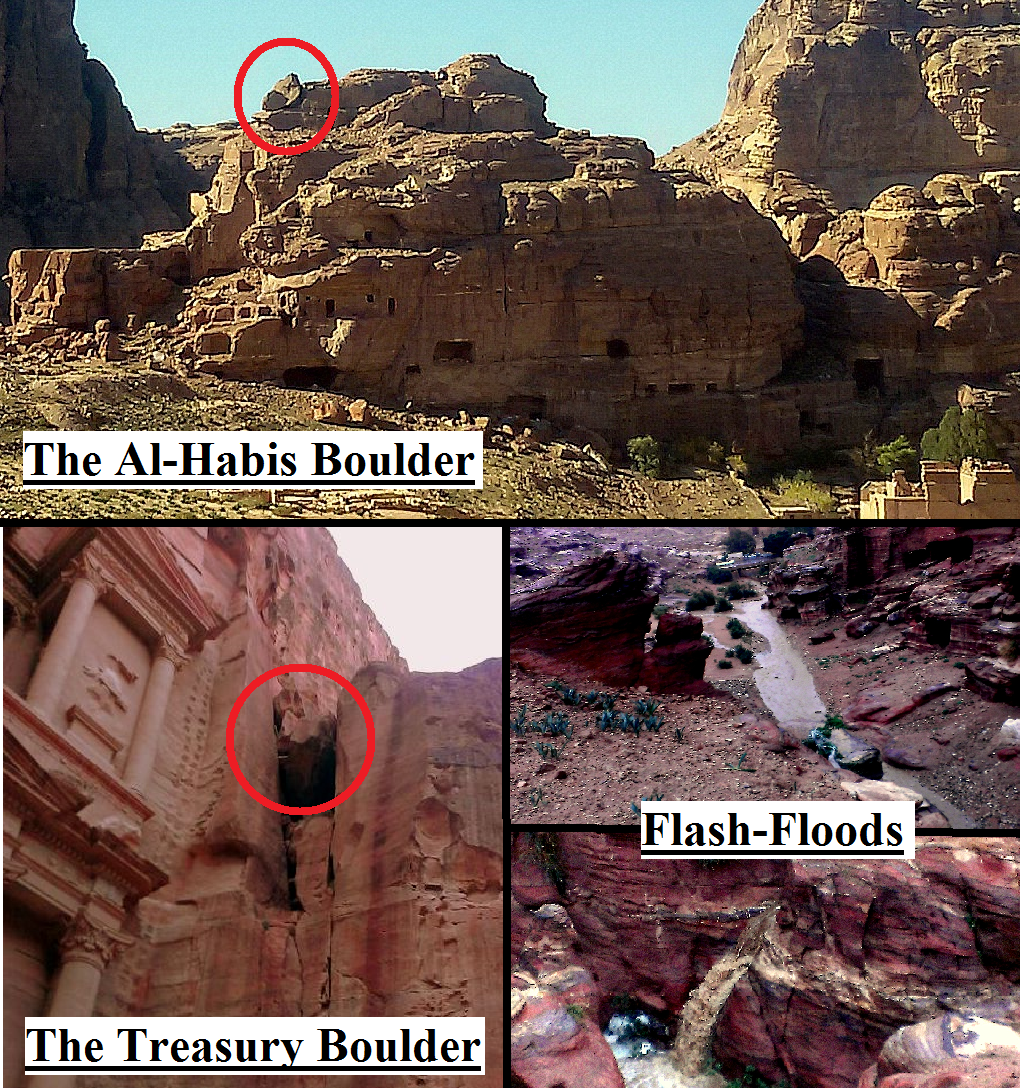
\includegraphics[width=\linewidth]{29-Verezen-figure02}
	\caption{The three natural and potential hazardous features.
		{\normalfont\scriptsize \\ \copyright\ by \shortauthor
	}}
	\label{fig:29-Verezen-figure02}
\end{figure}

The \IJSRAsubsection{Al-Habis Boulder} second natural feature is the boulder topping the Al-Habis mountain.
If this boulder falls downward in the East direction, it could tumble down the adjacent hill into archaeological structures and
tourist facilities.
This indicates a safety-risk in the case of dislocation caused by substantial forces such as earthquakes,
which are not uncommon in this region.
Petra has witnessed powerful earthquakes in the past, which inflicted great damage to its archaeology\footnote{Several earthquakes were recorded through history; this allows us to retrieve the years in which Petra has been subjected to extreme natural forces. Petra underwent devastating earthquakes in 31\BC, 114\AD, 363\AD, 551\AD, and 747\AD \parencites[63--64]{rababeh2014}[98--103]{peterman1994}.} \parencites[126]{alshawabkehy2010}[644]{heinrichs2008}.
Due to the Habis boulder’s unconsolidated state and the possibility of an earthquake,
it should be subjected to further risk-assessment and safety procedures. 

Throughout \IJSRAsubsection{Flash Floods} time, flash-floods are natural hazards occurring inside Petra and are known for
their destructive force and capability of removing significant amounts of debris \parencites[78--84]{franchi2009}[104]{ortloff2005}.
The debris-filled floods will affect any archaeological and natural sandstone in its path.
This force was observed during a field survey in the winter of 2014, when a rapidly formed flash-flood transported and deposited an ancient basalt grinder \pcref{fig:29-Verezen-figure03} and various large boulders.
The force and volume of the flash-flood depends on the amount of rainfall and surface run-off water supplied through
nine catchment areas located in the Petra area \parencites[171--172]{alweshahr1999}[130]{nichols2009}.
Flash-floods pose a major threat to people inside Petra; this was proven by the flash-flood of 1963,
which killed more than \num{20} French tourists \parencites[55--57]{comer2012}[55]{lingis2002}.

\begin{figure}[!htb]
	\includegraphics[width=\linewidth]{29-Verezen-figure03}
	\caption{An ancient basalt grinder transported and deposited by a flash-flood.
		{\normalfont\scriptsize \\ \copyright\ by \shortauthor
	}}
	\label{fig:29-Verezen-figure03}
\end{figure}

The \IJSRAsection{Discussion} results indicate that sandstone monuments and natural features in Petra are mainly susceptible to
physical weathering and detrimental circumstances such as; weather extremities, root-growth, flash-floods,
and human activities that are responsible for the abrasion and detachment of stone material, such as collapse, rock-falls, and
fissures  \parencites[267--284]{balaawi2011}[653]{heinrichs2008}[230]{turkington2005}.
The discussed natural features point to the presence of potential safety-risks in the archaeological park that
could threaten nearby archaeology, locals, and visitors.

Much is known about the various weathering factors in Petra as is attested by the numerous scholarly studies.
Unfortunately, many monuments in the archaeological park still lack protection, as was observed during the field-surveys in 2014 and 2015.
Most monuments are in dire need of protection and conservation, as is clear from presented case-studies in this paper.
In order to protect and preserve the chosen, and in fact all other, monuments, strict protection measures and
visitor regulations should be enforced.
In the presence of the ongoing weathering impacts, and without further preventive measures, the degradation and
consequential collapse of monuments is inevitable.
It is agreed by various scholars that risk- and damage-assessments are necessary to prevent further damage and
to safeguard Petra’s archaeology. One of those scholars, for example, is Tom Paradise who has argued:
\begin{IJSRAquote}{\cite[75]{paradise2010}}
		Moreover, the Jordanian government and regional Petra tourism council have developed plans to continually increase visitation across the valley. Therefore, in popular and susceptible tourist destinations like Petra, research that investigates natural and anthropogenic influences on architectural decay and envi¬ronmental degradation is essential before it is too late and irreversible changes have occurred in these vulnerable sites.
\end{IJSRAquote}

The condition of the Monastery’s Urn and the Corinthian Tomb both indicate the urgent need for attention and protection.
Additionally, the collapsed Tomb 609 makes clear that continuous damage-assessments throughout Petra are
required in order to safeguard Petra’s archaeology \parencite[672]{heinrichs2008}.
Several conservation works have been fulfilled in Petra however, not all are successful.
One unsuccessful attempt occurred at the Qasr-al Bint where structural parts were impregnated with
an incorrect mortar-type causing further damage.
This partially was due to the lack of a single conservation-policy in Jordan’s heritage sector which then led to
various unaligned conservation interventions.
Various mortar-types have negative and positive merits that should be kept in mind during
conservation works in Petra \parencite[926--932]{alsaad2001}.
Desalination techniques are available, which reduce salt-crystallization; however,
this needs improvement since some techniques increase decay \parencites[561--563]{matyscak2014}[1915--1916]{rörigdalgaard2015}[1125--1129]{young2003}.
Furthermore, the process of salt-weathering remains poorly understood and requires further research.
Currently, the ‘petraSalt’ research-project is aimed at gaining a better understanding of salt-weathering that may lead to
improved methods that reduce the impact of salt-weathering \parencite[347--348]{heinrichs2013a}.

\begin{figure}[!htb]
	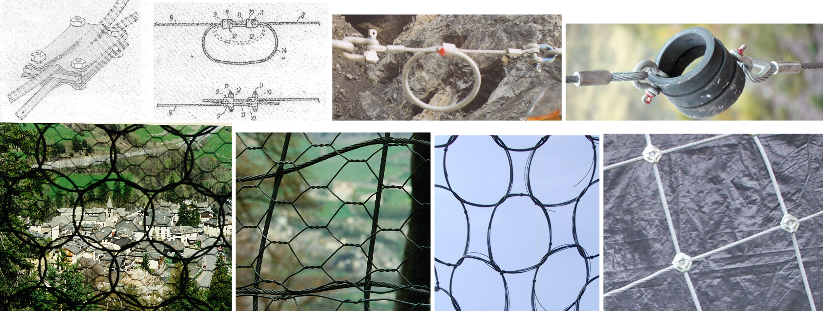
\includegraphics[width=\linewidth]{29-Verezen-figure04}
	\caption{An example of safety-measures.
		{\normalfont\scriptsize \\ \copyright\ by, and used with the permission of, Dr. Axel Volkwein
	}}
	\label{fig:29-Verezen-figure04}
\end{figure}

In regards to the chosen natural features, various options could contribute to maintain the safety for Petra’s archaeology and visitors,
such as steel-nets \pcref{fig:29-Verezen-figure04}, which retain falling debris during rock-falls \parencite[2638]{volkwein2011}.
The Al-Habis boulder and the Treasury’s boulder \pcref{fig:29-Verezen-figure02} are proofs of the silent, and often unnoticed,
presence of safety-risks and are just a glimpse of the collective amount of hazards in the park.
This suggests that extensive and continuous risk-assessments should be enforced in order to maintain a safe environment.
The rapid formation of flash-floods, after a rain- or snow-fall, likewise point to the need of the continuous monitoring of
weather patterns and its effect on Petra’s archaeological and natural features.

Concluding \IJSRAsection{Conclusion and Implications} from the information gained throughout this research,
direct attention is required for the selected monuments and natural features.
Previous studies have not highlighted architectural features of the monuments that were degraded and of potential safety risk.
This indicates the need for thorough damage-assessments of all and entire monuments including architectural features,
such as the Urn of the Monastery.
Likewise, a national conservation policy should help in achieving aligned conservation works in Petra \parencite[267--284]{balaawi2011}.

Regarding the protection of monuments, there should be an increased attention on reducing and researching salt-weathering and
on petrographic and geomorphological studies \parencite[347--348]{heinrichs2013a}.
Similar research, regarding salt-weathering, has been done at the sandstone Luxor Temple and
the Karnak Temple in Upper Egypt that are, similarly, in a severe state of degradation \parencite[1009--1102]{fhb03}.
Deterioration caused by continuous natural processes can be controlled through periodic damage-assessments and
the monitoring of weather-patterns in the region.
ICOMOS (2005) has published examinations on the impact of anthropogenic activity on Petra’s archaeology.
Based on these publications, a solid tourism- and
heritage-management plan for Petra could be designed \parencite[499--501]{comer2011}.
Furthermore, tourists should be prevented from climbing on monuments and scratching and writing on sandstone surfaces.
The placement of warning signage and the imposing of fines could prevent people from causing damage in
Petra \parencite[80--85]{mustafa2013}. 

Continuous risk-assessments of unconsolidated natural features, such as the Al-Habis and Treasury boulder, should be conducted.
Rock-fissures, which could lead to collapse, should be monitored and filled with
the correct mortar which should first be technically evaluated \parencite[926--932]{alsaad2001}.
Strict regulations regarding the allowance of visitors during significant rain- or snowfall should be applied to prevent dangerous situations.
As well, installing steel-safety nets \pcref{fig:29-Verezen-figure04} will contribute to the park’s safety in case of
rock-falls \parencite[2617--2639]{volkwein2011}.
Through the enforcement of safety regulations, protection measures, extensive risk- and damage-assessments and mapping affected monuments,
damage can be reduced and prevented \parencites[127]{alshawabkehy2010}[441--446]{delmonaco2013}.
If implemented, these options will contribute to the protection of Petra’s archaeology, visitors, and future;
and with that, the protection of irreplaceable and valuable data required to retrieve an understanding of this region’s past.

Hereby \IJSRAsection{Acknowledgments} I would like to thank Dr. Mark Driessen and Dr. Olivier Nieuwenhuysen. Both have been of great support in the process of conducting this research. Furthermore, many thanks go out to Gonzalo Linares, the executive editor of this journal, for kind guidance throughout the application process of this article. Additionally, I am thankful for the information provided by the ICOMOS, WMF, UNESCO and articles from various scholars just as concerned with the protection, safety and future of Petra. I am extremely grateful for all of those not mentioned here however, who likewise offered helpful advice and support throughout this research.

\begin{figure}[!htb]
	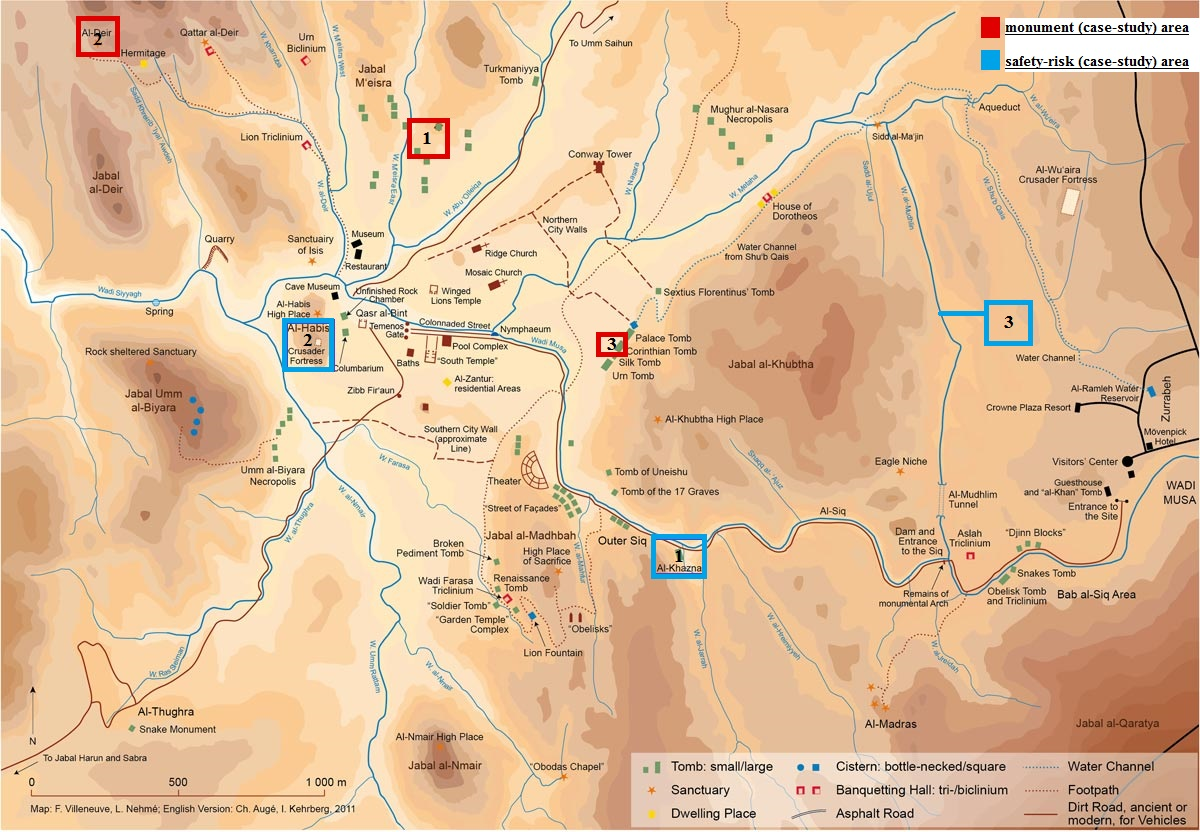
\includegraphics[width=\linewidth]{29-Verezen-figure-appendix02}
	\caption{Map of the Petra Archaeological Park (PAP).
		{\normalfont\scriptsize \\ Re-printed with permission from Nadine Meouchy (PhD), Head of the Presses de L’IFPO
	}}
	\label{fig:29-Verezen-figure-appendix02}
\end{figure}

\begin{figure}[!htb]
	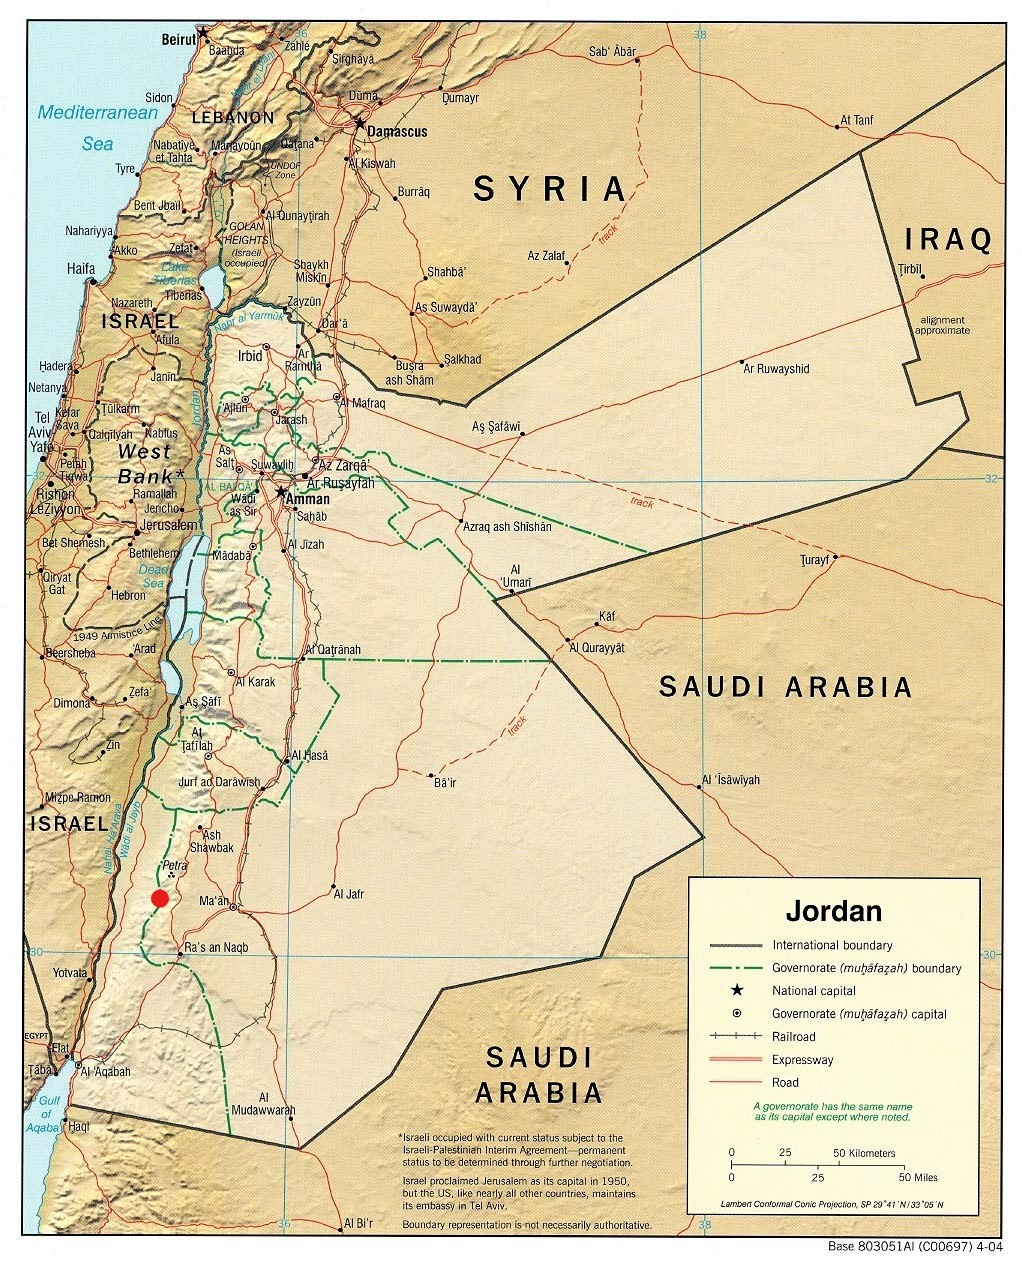
\includegraphics[width=\linewidth]{29-Verezen-figure-appendix01}
	\caption{Map of Jordan.
		{\normalfont\scriptsize \\ \copyright\ by The University of Texas Libraries, The University of Texas at Austin
	}}
	\label{fig:29-Verezen-figure-appendix01}
\end{figure}



\clearpage
%\nocite{*}%just for testing! Can be deleted
\IJSRAclosing%<---- don’t change this!